\chapter{尺度、弦与二十六维}

\lectureoverview{是什么决定了弦谱的间距？答案是张力，一个具有质量平方量纲的量。对于基本弦而言，这一观察将我们引向普朗克单位、直接激发的实际不可能性，以及强引力的出现。经过一段有意的中断之后，我们回到玻色开弦基态。对其零点能进行正规化，便给出了历史上那条\emph{容易}的途径，通向二十四个横向方向，从而通向二十六维时空。}

\section{我们此前略去的尺度}

到目前为止，我们谈论了振动和旋转的弦，却没有说明一个单位的激发意味着什么。一个强子可以被描绘成一根弦，它的振子可以被激发，但从一个态到下一个态的跃迁有多大？是什么决定了它？

在基本弦模型中只有一个有量纲的参数。要找到它，先从一根普通的拉伸弹簧开始。如果其两端相距\(\ell\)，胡克定律给出
\begin{equation}
  E_{\mathrm{spring}}=\frac{k\ell^2}{2}.
  \label{eq:l05-hooke}
\end{equation}
这个二分之一因子是在第一版写出之后由全班补上的。在这个开篇估计中，没有什么本质性的东西会依赖于这类数值因子。

\begin{figure}[H]
  \centering
  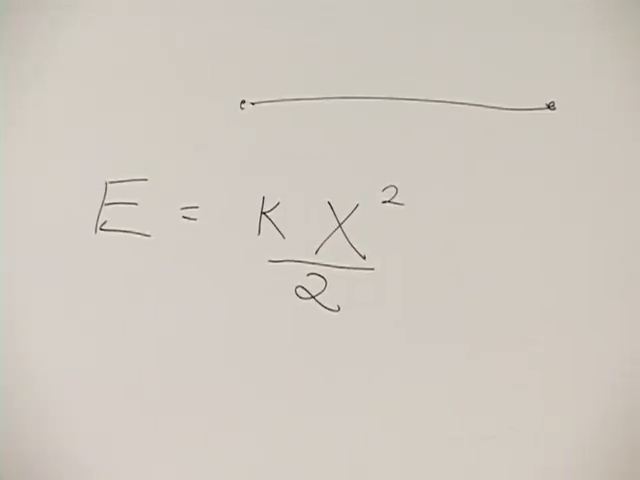
\includegraphics[width=0.72\textwidth]{lecture_05_figure_01.png}
  \caption{拉伸的线段及其胡克定律势能。}
  \lectureframe{00:02:28}
  \label{fig:l05-hooke-board}
\end{figure}

\eqref{eq:l05-hooke}中的能量是非相对论性的。在前几讲所用的无限动量描述中，内部非相对论能量并不正比于\(m\)，而是正比于\(m^2\)。因此我们示意性地写出
\begin{equation}
  m^2\sim k\ell^2,
  \qquad
  m\sim \sqrt{k}\,\ell.
  \label{eq:l05-mass-length}
\end{equation}
在弦的静止系中，其质量就是其能量，所以第二个关系式具有如下形式
\begin{equation}
  E_{\mathrm{rest}}\sim T_s\ell,
  \qquad
  T_s\equiv\sqrt{k}.
  \label{eq:l05-tension}
\end{equation}
系数\(T_s\)就是弦张力：单位长度所储存的能量。

\begin{figure}[H]
  \centering
  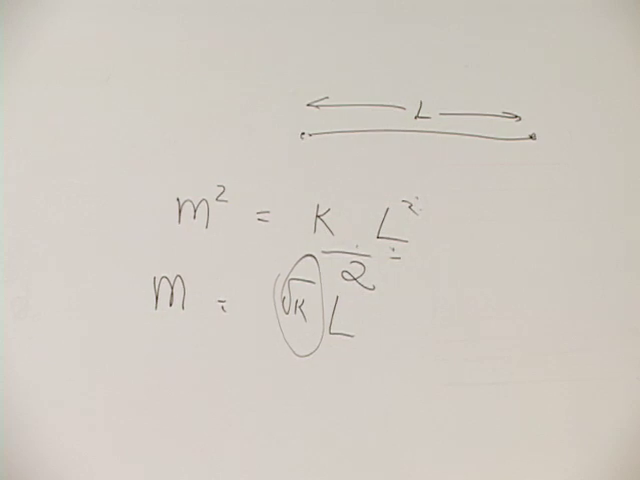
\includegraphics[width=0.78\textwidth]{lecture_05_figure_02.png}
  \caption{黑板从\(m^2\sim k\ell^2\)过渡到正比于长度的质量。}
  \lectureframe{00:05:42}
  \label{fig:l05-mass-length-board}
\end{figure}

这套记号是为本讲的弹簧类比而改写的。在标准的相对论性弦记号中，人们通常写出
\begin{equation}
  T_s=\frac{1}{2\pi\alpha'},
  \label{eq:l05-alpha-prime}
\end{equation}
于是弦能级的增量产生量级为\(1/\alpha'\)的\(m^2\)增量，等价地说，量级为张力。
\editorialnote{本讲中有效的\(k\)被选得使\(\sqrt{k}\)扮演张力的角色。与约定无关的陈述是：\(T_s\)具有质量平方的量纲，并且雷吉斜率满足\(\alpha'\propto T_s^{-1}\)。}

\subsection{量纲与振子能隙}

令\(c=\hbar=1\)。能量于是具有长度倒数的量纲：
\begin{equation}
  [E]=L^{-1}.
\end{equation}
由于张力是单位长度的能量，
\begin{equation}
  [T_s]=L^{-2}=E^2.
  \label{eq:l05-tension-dimension}
\end{equation}
这就是为什么弦谱自然地以质量平方为间距。

\begin{figure}[H]
  \centering
  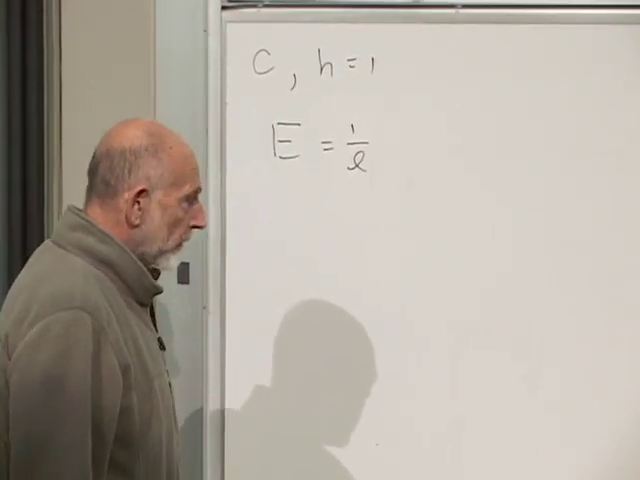
\includegraphics[width=0.68\textwidth]{lecture_05_figure_03.png}
  \caption{黑板上的自然单位：\(c=\hbar=1\)，能量是长度倒数，而振子频率由弹簧尺度控制。}
  \lectureframe{00:06:05}
  \label{fig:l05-natural-units-board}
\end{figure}

普通的振子从另一个方向说明了同一点。对于质量为\(\mu\)的弹簧，
\begin{equation}
  \omega=\sqrt{\frac{k}{\mu}},
  \qquad
  \Delta E=\hbar\omega.
\end{equation}
更硬的弹簧有更高的频率和更大的量子能隙。一根弦包含无穷多个这样的简正模，但它们的共同尺度由\(T_s\)固定。一旦张力已知，弦谱的间距也就已知了。

张力也具有力的量纲，因为力乘以距离就是能量。想象把一端固定，从另一端悬挂一个重物。一根满足\(E=T_s\ell\)的理想相对论性弦能够支撑一个由\(T_s\)设定的力，与它的长度无关。在这个刻意虚构的比较中，由观测到的激发能推断出的强子张力，相当于一辆卡车的重量。从来没有卡车被悬挂在介子上；测得的谱给出张力，而张力给出这一力学比较。

基本弦会硬得多。如果它们构成了电子、光子和引力子的基础，那么它们的第一次振子激发必定远高于观测到的粒子能量。在同一个虚构的引力实验中，它们的张力可以支撑星系量级的东西。这一比较的要点不在于工程。而在于：巨大的张力既意味着很大的激发能，也意味着极小的基态涨落。

\section{由普适常数构成的单位}

多大的尺度才算足够巨大？自然的基准是普朗克尺度。与其引用它，不如让我们把它构造出来。

米、千克和秒是极好的实验室单位，但它们的起源却是人体尺度。米适合量布或绳子；英尺得名于身体的一部分；秒则是一天的可操作分数。人们可以把质子半径设为1，从而简化某些核公式，但质子只是一种特定的复合粒子。这样的选择不会简化整个物理学。

三个量纲常数具有更普遍的作用范围：
\begin{itemize}
  \item \(c\) 为每个物质系统设定了极限速度；
  \item \(\hbar\) 出现在每个量子系统的不确定关系之中；
  \item \(G\) 将引力与每一种形式的质能耦合起来。
\end{itemize}
选择使 \(c=\hbar=G=1\) 的单位，等价于由这些常数构造出长度、时间和质量的单位。

它们的通常量纲为
\begin{equation}
  \begin{aligned}
    [c]&=LT^{-1},
    & [\hbar]&=ML^2T^{-1},\\
    [G]&=L^3M^{-1}T^{-2}.
  \end{aligned}
  \label{eq:l05-dimensions-constants}
\end{equation}
中间的关系直接来自
\(\Delta x\,\Delta p\gtrsim\hbar\)。最后一条则例如来自
\begin{equation}
  a=\frac{GM}{r^2}.
\end{equation}

\begin{figure}[H]
  \centering
  \begin{minipage}[t]{0.48\textwidth}
    \centering
    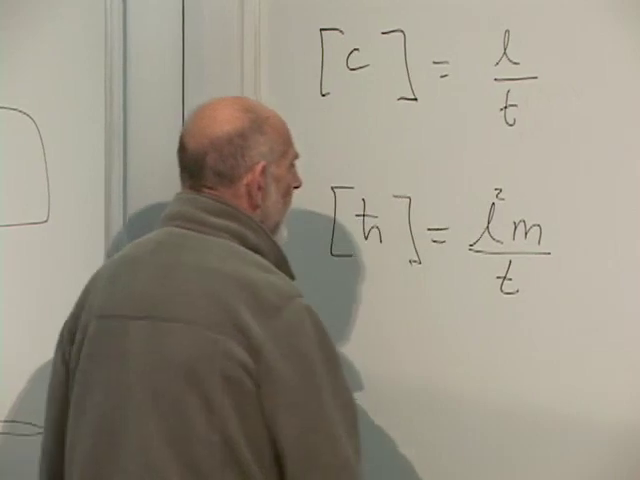
\includegraphics[width=\textwidth]{lecture_05_figure_04.png}
    \par\smallskip\footnotesize (a) \(c\) 和 \(\hbar\) 的单位。
  \end{minipage}\hfill
  \begin{minipage}[t]{0.48\textwidth}
    \centering
    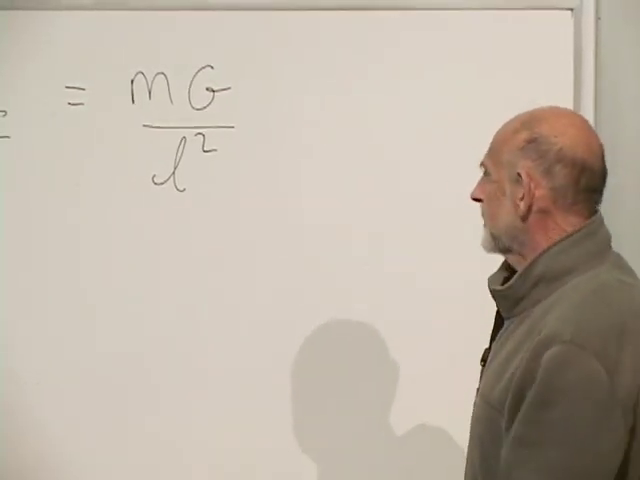
\includegraphics[width=\textwidth]{lecture_05_figure_05.png}
    \par\smallskip\footnotesize (b) 由牛顿加速度得到的 \(G\) 的单位。
  \end{minipage}
  \caption{课堂上汇集起来的量纲分析要素。}
  \lectureframe{00:25:43--00:26:40}
  \label{fig:l05-dimensional-analysis-board}
\end{figure}

\subsection{普朗克面积优先}

寻找幂次 \(p,q,r\)，使得
\begin{equation}
  G^p\hbar^q c^r
\end{equation}
具有量纲 \(L^2\)。优先选择面积可以避免过早出现平方根，也预示了面积日后在引力中将扮演的特殊角色。由
\eqref{eq:l05-dimensions-constants}，质量和时间的抵消给出
\begin{equation}
  -p+q=0,
  \qquad
  -2p-q-r=0.
\end{equation}
剩余的长度幂次必须满足
\begin{equation}
  3p+2q+r=2.
\end{equation}
因此 \(q=p\)、\(r=-3p\) 和 \(p=1\)。普朗克面积为
\begin{equation}
  \ell_P^2=\frac{G\hbar}{c^3},
  \label{eq:l05-planck-area}
\end{equation}
从而
\begin{equation}
  \ell_P=\sqrt{\frac{G\hbar}{c^3}},
  \qquad
  t_P=\frac{\ell_P}{c},
  \qquad
  m_P=\sqrt{\frac{\hbar c}{G}}.
  \label{eq:l05-planck-units}
\end{equation}

\begin{figure}[H]
  \centering
  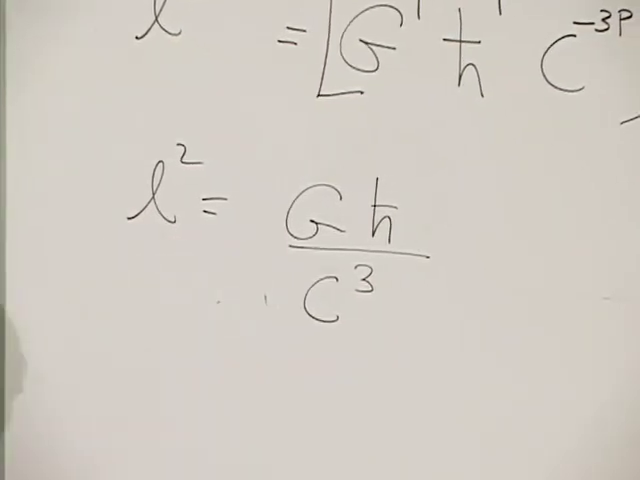
\includegraphics[width=0.78\textwidth]{lecture_05_figure_06.png}
  \caption{关于普朗克面积和长度的完整量纲论证。}
  \lectureframe{00:31:34}
  \label{fig:l05-planck-area-board}
\end{figure}

在数量级精度下，
\begin{equation}
  \begin{aligned}
    \ell_P&\sim10^{-35}\,\mathrm{m},
    &t_P&\sim10^{-43}\,\mathrm{s},\\
    m_P&\sim10^{-8}\,\mathrm{kg},
    &m_Pc^2&\sim10^{19}\,\mathrm{GeV}.
  \end{aligned}
  \label{eq:l05-planck-numbers}
\end{equation}

\begin{figure}[H]
  \centering
  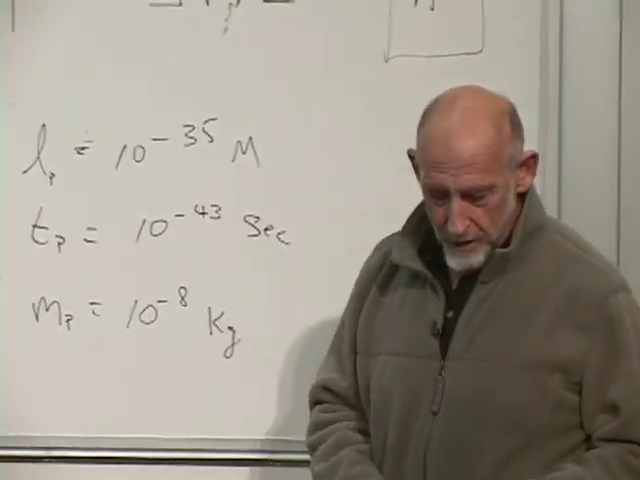
\includegraphics[width=0.72\textwidth]{lecture_05_figure_07.png}
  \caption{按数量级记录下来的三个普朗克尺度。}
  \lectureframe{00:35:12}
  \label{fig:l05-planck-values-board}
\end{figure}

长度和时间小得无法想象，而质量按粒子标准来看却大得惊人，大致相当于一粒细尘埃的质量。它的静能约为几吉焦，与一箱汽油中的化学能相当。相比之下，可观测宇宙大约跨越 \(10^{60}\) 个普朗克长度，并且已经存在了大约 \(10^{60}\) 个普朗克时间。这些比较意在赋予这些单位以物理分量，而不是提高它们的数值精度。

如果特征弦长 \(\ell_s=\sqrt{\alpha'}\) 接近 \(\ell_P\)，那么弦的量子尺度就接近 \(\ell_P\)，其振动周期接近 \(t_P\)，而其第一个有质量激发接近 \(m_P\)。讲座允许十倍、一百倍甚至更大的因子；这一认定是一种预期，而不是量纲恒等式。

\begin{classroomqa}
\audiencequestion{普朗克尺度质量是粒子基态之上的增量吗？\lecturetimestamp{00:38:37}}
\lecturerresponse{等间距的量是质量的平方。如果基态很轻，那么第一个弦激发的 \(m^2\) 会大出 \(m_P^2\) 量级的一个量，因此它的质量和所需的质心能量都在 \(m_P\) 量级。}
\end{classroomqa}

\section{两个尺度应当有多接近？}

\begin{classroomqa}
\audiencequestion{量纲分析给出 \(\ell_P\)，但为什么那个数就应该是弦的长度？\lecturetimestamp{00:40:21}}
\lecturerresponse{这是一个由引力和未观测到弦结构这一事实所支持的物理猜测，而不是仅由量纲分析得出的结论。弦长可能大于普朗克长度，这意味着其能标更低。讲座只论证了它不应是普通的粒子物理长度，并且把它压到远低于普朗克长度会遭遇引力坍缩。}
\end{classroomqa}

两个尺度之间的关系实际上依赖于耦合。在一个完整的紧致化中，\(\ell_P\)、\(\ell_s\)、弦耦合以及紧致化体积会一起进入。并不存在普适方程 \(\ell_s=\ell_P\)。讲座中留存下来的是尺度论证：弦效应必须在非常高的能标进入，而亚普朗克尺度的局域化不能在忽略引力的情况下讨论。
\editorialnote{现代弦构造不必把弦长与四维普朗克长度完全等同起来。它们的关系取决于弦耦合和紧致化数据。}

\begin{classroomqa}
\audiencequestion{如果把普朗克长度视为最小的有用长度，那么普朗克质量是否也是可能的最小质量？\lecturetimestamp{00:43:27}}
\lecturerresponse{不是。普通粒子要轻得多。普朗克质量是这样一个尺度：在此尺度下，一个致密物体的引力半径可以与其量子波长相当。用讲座中的启发式语言来说，它是最轻的半经典黑洞的尺度，其寿命为普朗克时间量级；最后这句话不应被误认为是对一个完全量子化物体的精确描述。}
\end{classroomqa}

\subsection{跑动耦合能告诉我们什么}

有间接证据表明，传统量子场论在远超加速器直接可达范围的尺度上仍然有效。三种标准模型规范耦合在可及能量下被测量，它们的尺度依赖性可以被外推。在讲座的示意图中，\(U(1)\)、\(SU(2)\)和\(SU(3)\)耦合在一个高统一尺度处彼此接近，该尺度也许比普朗克能量低几个数量级。

\begin{figure}[H]
  \centering
  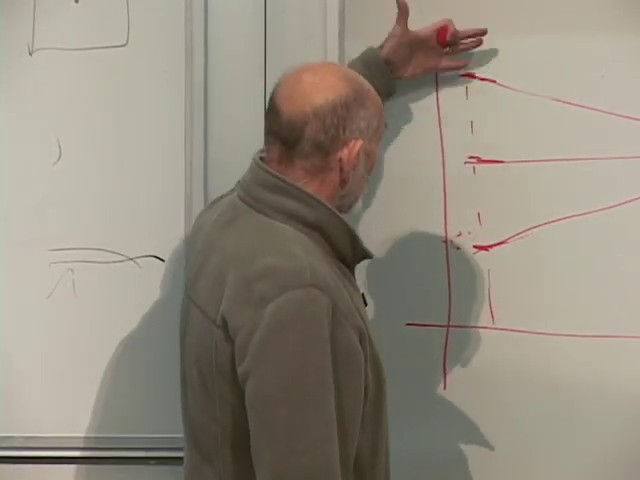
\includegraphics[width=0.70\textwidth]{lecture_05_figure_08.png}
  \caption{示意性的跑动耦合图。三条规范曲线在上升的引力强度变为量级一之前彼此接近。}
  \lectureframe{00:47:18}
  \label{fig:l05-running-couplings-board}
\end{figure}

这是外推，而不是在交叉点处的直接实验。实验室能量与统一能量之间的额外粒子或阈值可以改变斜率。谨慎的结论只是：已知场论在普通距离上没有显示出弦尺度子结构的迹象，而一个合理的弦尺度位于所推断的统一尺度与普朗克尺度之间的巨大区间中的某处。

\begin{classroomqa}
\audiencequestion{正在被外推的是哪三种耦合？\lecturetimestamp{00:48:28}}
\lecturerresponse{它们是与\(U(1)\)、\(SU(2)\)和\(SU(3)\)相关的规范耦合：超荷、弱和强相互作用。电磁作用从电弱混合中涌现，而不是在这一账目中作为一个独立的第四规范因子。}
\end{classroomqa}

\begin{classroomqa}
\audiencequestion{引力常数\(G\)本身会随着我们探测更高能量而增大吗？\lecturetimestamp{00:49:30}}
\lecturerresponse{\(G\)是有量纲的，因此它本身并不是与无量纲规范耦合相比较的正确量。在特征能量\(M\)下，无量纲引力强度示意性地表现为\(GM^2/(\hbar c)\)。该组合随能量增大，并在普朗克尺度处变为量级一。}
\end{classroomqa}

力律使这一比较变得可见：
\begin{equation}
  F_{\mathrm{em}}\sim\frac{e^2}{r^2},
  \qquad
  F_{\mathrm{grav}}\sim\frac{GM^2}{r^2}.
  \label{eq:l05-force-laws}
\end{equation}
因此，\(e^2\)不是与\(G\)比较，而是与自然单位下的\(GM^2\)比较。

\begin{figure}[H]
  \centering
  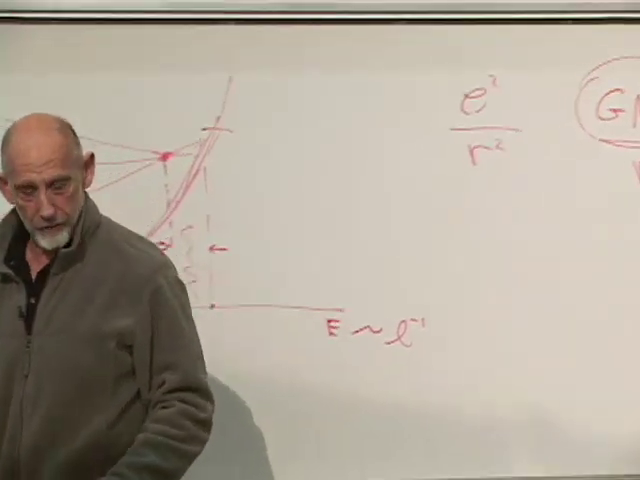
\includegraphics[width=0.74\textwidth]{lecture_05_figure_09.png}
  \caption{用于确定无量纲引力强度的电磁力律与引力力律。}
  \lectureframe{00:50:50}
  \label{fig:l05-force-laws-board}
\end{figure}

\section{为什么直接弦谱学遥不可及}

我们如何通过实验确立电子是一根弦？我们会做强子谱学做过的事：足够猛烈地撞击它，以激发其内部模式，并寻找一个质量遵循弦模式的态塔。如果第一个有质量能级位于\(10^{19}\,\mathrm{GeV}\)附近，那也远超任何直接机器。

总能量并不是唯一的障碍。它还必须被集中在极小的碰撞参数内。这就引出了黑洞。

\begin{classroomqa}
\audiencequestion{在这些能量下，加速器会开始产生小黑洞吗？\lecturetimestamp{00:50:57}}
\lecturerresponse{一旦质心能量被集中在引力半径之内，这就是启发式的预期。恒星黑洞是由引力势能挤压一颗大质量恒星而形成的。微观黑洞则相反，是由动能聚焦到微小碰撞区域而形成的。在四维引力中，所需尺度是普朗克量级。}
\end{classroomqa}

为了提供参照，直线加速器的能量增益大致与其长度成正比。讲座以大约两英里对应大约\(100\,\mathrm{GeV}\)作为简单的SLAC尺度标尺。若以相同梯度达到\(10^{19}\,\mathrm{GeV}\)，长度将乘以大约\(10^{17}\)，从而产生一台星系尺度的机器。

即便这样一台机器也需要光度。束流并不是一次一对地以普朗克长度精度瞄准；而是数量巨大的粒子交叉通过，使得少数粒子在所需碰撞参数下碰撞。将普朗克能量乘以巨大的碰撞率，会产生同样荒谬的功率需求。这些估计是有意粗略的，但其结论是稳定的：在普朗克尺度上进行直接弦谱学并不是一个能够合理设计的实验。

间接证据必须更具结构性：一种能够以足够的具体性给出所观测到的低能粒子与相互作用、从而可被检验的理论，或者紧致化效应在远低于弦尺度的能标下仍然存活。本讲并不声称这样一种决定性的构造已经掌握在手。

\subsection{额外维度与定域化极限}

\begin{classroomqa}
\audiencequestion{额外维度的大小是否也接近普朗克长度？\lecturetimestamp{00:56:23}}
\lecturerresponse{在这一基本图像中，它们预期是极其微小的，尽管这一论证并未将其精确固定。如果某个紧致维度大到足以在较低能量下被探测，那么新的 Kaluza--Klein 模式以及更高维的行为早就应当改变我们所观测到的场论了。因此，该场论的成功外推为这类维度给出了一个上界。}
\end{classroomqa}

\begin{classroomqa}
\audiencequestion{为什么弦或紧致维度不可能比 \(\ell_P\) 小许多个数量级？\lecturetimestamp{00:57:48}}
\lecturerresponse{分辨更短的距离需要更大的动量。超过普朗克尺度之后，定域化所需的能量其引力半径与被探测的区域相当，继而变得比该区域更大。实验在分辨出更小的普通弦之前，就已经制造出了一个黑洞。}
\end{classroomqa}

不确定性原理给出了这一估计。要定域化到 \(\Delta x\)，需要

\begin{classroomqa}
\audiencequestion{一旦选定了普朗克长度与普朗克时间，普朗克质量是如何在物理上被确定的？\lecturetimestamp{00:59:04}}
\lecturerresponse{使用 \(\hbar\) 或 \(G\) 将长度尺度换算为能量。不确定性原理表明，将两个粒子定域化在 \(\ell_P\) 之内需要量级为 \(\hbar/\ell_P\) 的动量，因而需要量级为 \(m_Pc^2\) 的能量。等价地说，它就是使量子长度与引力长度变得相当的那个质量。}
\end{classroomqa}

\begin{equation}
  \Delta p\gtrsim\frac{\hbar}{\Delta x},
  \qquad
  E\sim c\,\Delta p.
  \label{eq:l05-localization}
\end{equation}
在 \(\Delta x=\ell_P\) 处，该能量为
\begin{equation}
  E\sim\frac{\hbar c}{\ell_P}=m_Pc^2.
\end{equation}
与此同时，施瓦西半径
\begin{equation}
  r_s\sim\frac{GE}{c^4}
\end{equation}
在量级上为 \(\ell_P\)，相差若干数值常数。量子定域化与引力坍缩在同一尺度上相遇。

\begin{figure}[H]
  \centering
  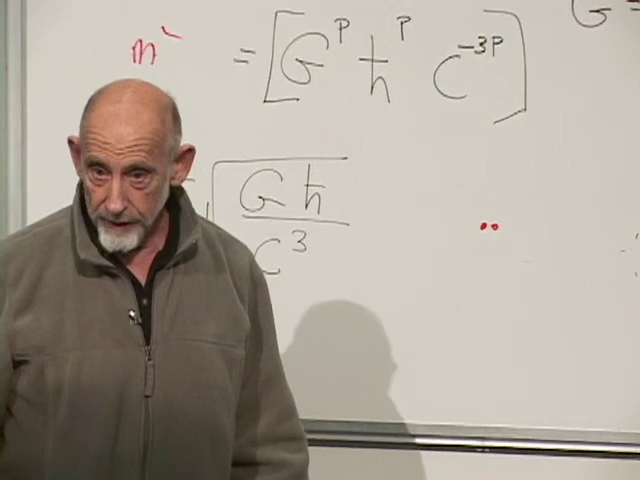
\includegraphics[width=0.74\textwidth]{lecture_05_figure_10.png}
  \caption{在定域化论证过程中重新审视的普朗克长度与质量公式。}
  \lectureframe{01:00:25}
  \label{fig:l05-localization-board}
\end{figure}

至此，尺度设定论证完成。

\section{基态必须位于光子之下}

休息之后有两条可能的方向：开始讲共形变换，或者给出通往临界维数的更古老、更容易的途径。我们选择后者，并附上一句警告。这条容易的论证并不容易，而且它也不是最深刻的理由。尽管如此，它是正确的，并且接近历史上的发现。

回到开弦玻色弦。用横向产生算符作用一次会产生两个极化态。由于不存在纵向的第三个态，该激发必须是一个无质量矢量。在取一个模式-\(1\) 量子使 \(m^2\) 升高一个单位的单位制下，
\begin{equation}
  m_{\mathrm{ground}}^2=-1,
  \qquad
  m_{\mathrm{first}}^2=-1+1=0.
  \label{eq:l05-open-intercept}
\end{equation}
快子基态仍然是玻色弦理论的一个问题；它被承认并暂时搁置。眼下的问题是 \eqref{eq:l05-open-intercept} 中的负单位从何而来。

每个弦模式都是一个谐振子。取 \(\hbar=1\)，其真空能量为
\begin{equation}
  E_{0,n}=\frac{\omega_n}{2}.
\end{equation}
对于弦，\(\omega_n=n\)，因此一个横向坐标形式上贡献
\begin{equation}
  E_0^{(1)}
  =\frac12\sum_{n=1}^{\infty}n.
  \label{eq:l05-formal-zero-point}
\end{equation}

\begin{figure}[H]
  \centering
  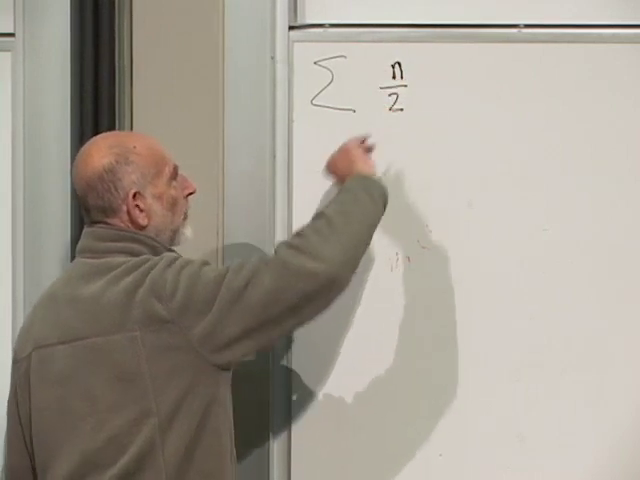
\includegraphics[width=0.70\textwidth]{lecture_05_figure_11.png}
  \caption{在回顾了模式频率之后写出的零点求和 \(\sum n/2\)。}
  \lectureframe{01:06:18}
  \label{fig:l05-zero-point-board}
\end{figure}

现在困难变得尖锐了。
\eqref{eq:l05-formal-zero-point} 中的每一项都是正的，而且该求和发散。它如何能给出一个有限的负截距？

\section{在读取谱之前先减去运动}

在对该求和进行正规化之前，回顾一下为什么内能会被等同于质量平方。对于一个携带大纵向动量 \(P>0\) 的粒子，
\begin{equation}
  E=\sqrt{P^2+m^2}
   =P+\frac{m^2}{2P}
   +O(P^{-3}).
  \label{eq:l05-large-p-energy}
\end{equation}

\begin{figure}[H]
  \centering
  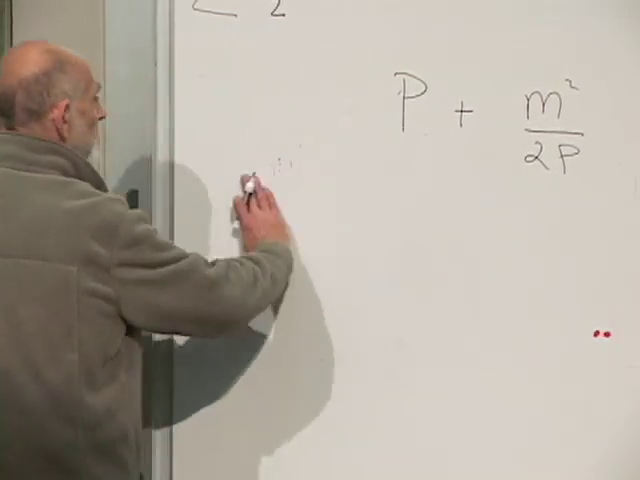
\includegraphics[width=0.70\textwidth]{lecture_05_figure_12.png}
  \caption{将整体动量与内部质量项分离开来的大-\(P\) 展开。}
  \lectureframe{01:07:35}
  \label{fig:l05-fast-energy-board}
\end{figure}

第一项是沿 \(z\) 轴的无趣的整体运动。它是守恒的，并且对于所有具有相同 \(P\) 的内部态都是共同的。减去它并重新标度，就消去了运动学上的时间膨胀：
\begin{equation}
  \begin{aligned}
    E-P&=\frac{m^2}{2P}+O(P^{-3}),\\
    2P(E-P)&=m^2+O(P^{-2}).
  \end{aligned}
  \label{eq:l05-internal-energy}
\end{equation}

原子提供了物理图像。对氢原子进行助推。它的总能量增大，但两个内部能级之间的能量差，按实验室时间测量，却缩小了，因为原子的时钟发生了膨胀。\eqref{eq:l05-large-p-energy} 中的因子 \(1/P\) 就是这种压低。乘以 \(2P\) 便恢复了不变的质量平方差。

因此，裸基态能量不必字面上就是 \(-1\)。它可能包含一个与整体纵向能量相关的大块状态无关部分，再加上一个有限的内禀剩余部分。讲义重写了助推后的关系式，以展示这两部分，然后才转回振子求和。

\begin{figure}[H]
  \centering
  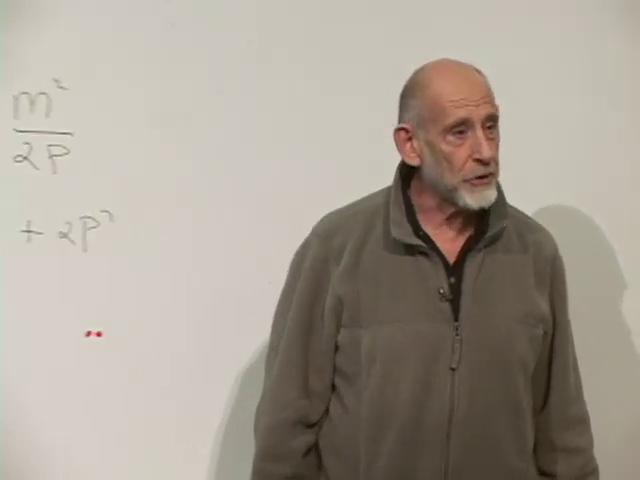
\includegraphics[width=0.76\textwidth]{lecture_05_figure_13.png}
  \caption{与大的状态无关纵向贡献并列展示的不变质量项。}
  \lectureframe{01:11:34}
  \label{fig:l05-infinite-piece-board}
\end{figure}

无穷大的真空能量在量子场论中是熟悉的。人们常常把一个发散的状态无关常数与可观测的能量差分开。讲义将此与房间中电磁场的零点能相比较，并坦率地称这一做法不能令人满意，但却是标准的。这里我们遵循同样的启发式做法：分离出发散部分，并追问是否留下一个确定的有限剩余。

\section{对求和进行正规化}

引入一个正的正规化因子 \(\epsilon\)：
\begin{equation}
  S_1(\epsilon)
  =\sum_{n=1}^{\infty}n e^{-n\epsilon}.
  \label{eq:l05-regulated-sum}
\end{equation}
对每个 \(\epsilon>0\)，指数最终会压倒因子 \(n\)，因此该求和收敛。让 \(\epsilon\) 趋于零便去掉了截断。

\begin{figure}[H]
  \centering
  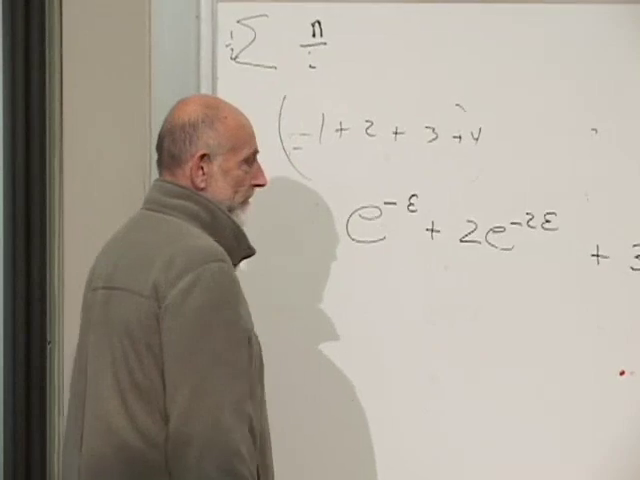
\includegraphics[width=0.78\textwidth]{lecture_05_figure_14.png}
  \caption{逐项施加于 \(1+2+3+\cdots\) 的指数正规化因子。}
  \lectureframe{01:16:42}
  \label{fig:l05-regulator-board}
\end{figure}

因子 \(n\) 可以通过微分生成：
\begin{equation}
  S_1(\epsilon)
  =
  -\frac{d}{d\epsilon}
  \sum_{n=1}^{\infty}e^{-n\epsilon}.
  \label{eq:l05-derivative-trick}
\end{equation}

\begin{figure}[H]
  \centering
  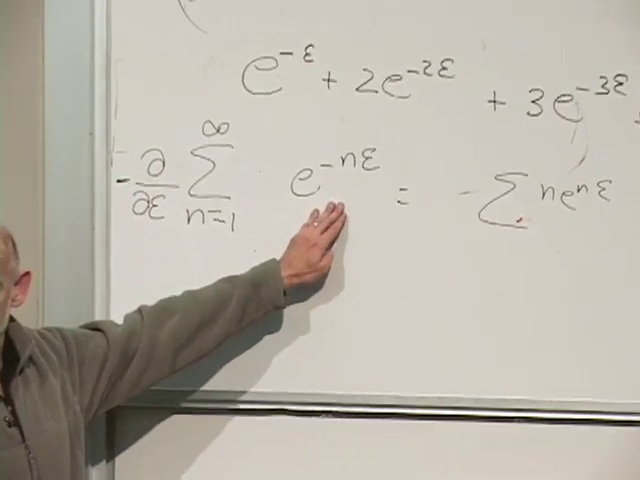
\includegraphics[width=0.76\textwidth]{lecture_05_figure_15.png}
  \caption{对截断参数求导会带下 \(-n\)。}
  \lectureframe{01:18:05}
  \label{fig:l05-derivative-board}
\end{figure}

剩下的级数是几何级数：
\begin{equation}
  S_0(\epsilon)
  \equiv
  \sum_{n=1}^{\infty}e^{-n\epsilon}
  =
  \frac{e^{-\epsilon}}{1-e^{-\epsilon}}
  =
  \frac{1}{e^\epsilon-1}.
  \label{eq:l05-geometric-sum}
\end{equation}

\begin{figure}[H]
  \centering
  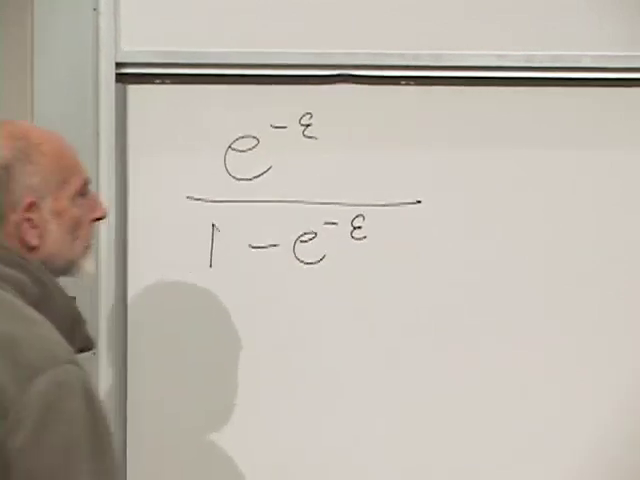
\includegraphics[width=0.68\textwidth]{lecture_05_figure_16.png}
  \caption{正规化后的几何级数的闭式形式。}
  \lectureframe{01:19:12}
  \label{fig:l05-geometric-board}
\end{figure}

在小的 \(\epsilon\) 处展开：
\begin{equation}
  S_0(\epsilon)
  =
  \frac{1}{\epsilon}
  -\frac12
  +\frac{\epsilon}{12}
  -\frac{\epsilon^3}{720}
  +O(\epsilon^5).
  \label{eq:l05-bernoulli-expansion}
\end{equation}
板书是通过分别展开分子和分母、提出一个 \(\epsilon\) 的幂、然后展开倒数而得到这一结果的。该计算包含若干课堂上的符号检查；紧凑表达式 \eqref{eq:l05-bernoulli-expansion} 是其整理后的结果。

\begin{figure}[H]
  \centering
  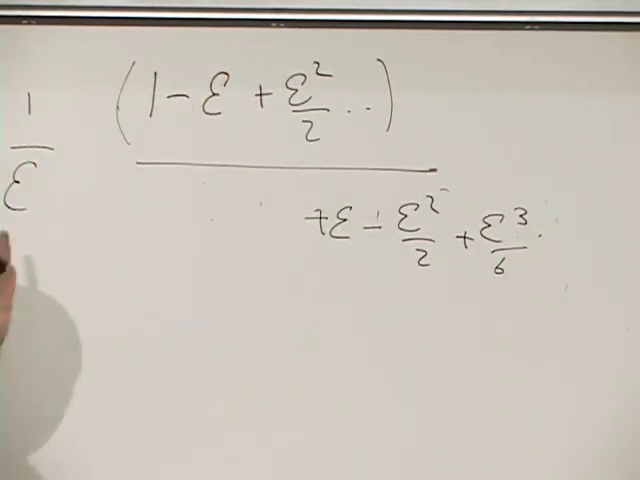
\includegraphics[width=0.78\textwidth]{lecture_05_figure_17.png}
  \caption{在简化倒数之前的分子和分母展开。}
  \lectureframe{01:23:10}
  \label{fig:l05-expansion-board}
\end{figure}

施加 \(-d/d\epsilon\) 得到
\begin{equation}
  S_1(\epsilon)
  =
  \frac{1}{\epsilon^2}
  -\frac{1}{12}
  +\frac{\epsilon^2}{240}
  +O(\epsilon^4).
  \label{eq:l05-regulated-result}
\end{equation}

\begin{figure}[H]
  \centering
  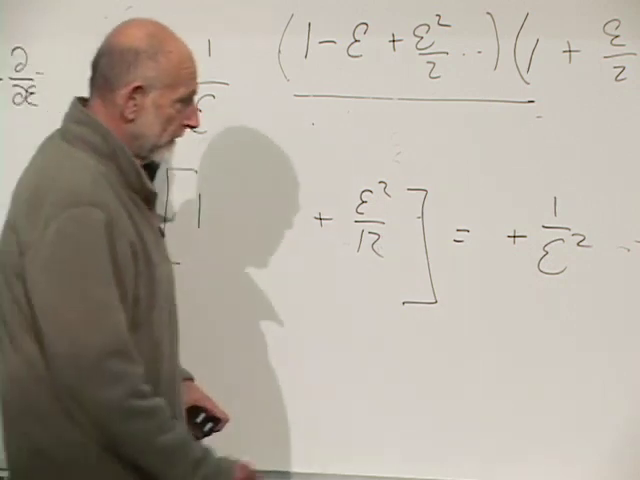
\includegraphics[width=0.78\textwidth]{lecture_05_figure_18.png}
  \caption{正规化计算末尾的发散 \(1/\epsilon^2\) 项和有限 \(-1/12\) 剩余。}
  \lectureframe{01:29:48}
  \label{fig:l05-minus-twelve-board}
\end{figure}

人们常开玩笑地把这一结果概括为
\(1+2+3+\cdots=-1/12\)。这并不是通常意义下的收敛。方程
\eqref{eq:l05-regulated-result} 表明，这个特定的正规化因子产生一个发散项加上一个与正规化因子无关的有限部分：
\begin{equation}
  \underbrace{\frac{1}{\epsilon^2}}_{\text{divergent}}
  \;+\;
  \underbrace{\left(-\frac{1}{12}\right)}_{\text{finite}}
  \;+\;O(\epsilon^2).
\end{equation}
讲义把第一项吸收进已经存在的状态无关部分，并保留第二项。它还保留了归因于泡利的警告：无穷大本身并不使一个量成为零。一个自洽的理论必须解释为什么允许做这种减法。

在
\eqref{eq:l05-formal-zero-point} 中恢复二分之一这个因子，一个横向坐标贡献
\begin{equation}
  E_0^{(1)}=-\frac{1}{24}.
  \label{eq:l05-one-transverse-zero-point}
\end{equation}

\begin{figure}[H]
  \centering
  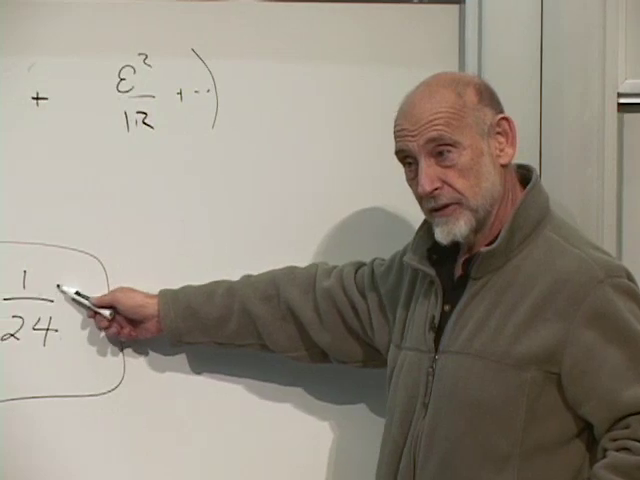
\includegraphics[width=0.68\textwidth]{lecture_05_figure_19.png}
  \caption{二分之一这个因子把有限的
  \(-1/12\) 转换为每个横向坐标的 \(-1/24\)。}
  \lectureframe{01:33:42}
  \label{fig:l05-minus-twenty-four-board}
\end{figure}

\section{数横向方向}

设 \(D_\perp\) 为横向弦坐标的数目。它们的总真空贡献为
\begin{equation}
  E_0^{\mathrm{open}}
  =-\frac{D_\perp}{24}.
  \label{eq:l05-open-vacuum}
\end{equation}
为了使第一个开弦振子把基态从
\(-1\) 提升到无质量能级，我们需要
\begin{equation}
  -\frac{D_\perp}{24}=-1.
\end{equation}
因此
\begin{equation}
  D_\perp=24.
\end{equation}
这些就是垂直于大纵向动量的方向。加上那个纵向空间方向和时间，得到
\begin{equation}
  D=D_\perp+2=26.
  \label{eq:l05-critical-dimension}
\end{equation}

\begin{classroomqa}
\audiencequestion{这个论证是何时进入弦理论的？\lecturetimestamp{01:35:27}}
\lecturerresponse{它属于最初强子弦的时代，大约在
1969 年和 1970 年代初。雷吉轨迹当时已在实验上为人所知。一旦振子模型被独立地探索，人们就发现第一激发态具有两个而非三个矢量极化，从而迫使它无质量。所需的截距随即迅速导致二十四个横向振子。}
\end{classroomqa}

在当时，这看起来几乎奇怪得令人难以置信。一个正规化后的真空求和为什么应当知道时空的维度？然而各个部分彼此吻合：无质量矢量、截距和横向振子数目都选出了同一个数。

\subsection{闭弦检验这个计数}

一根闭弦需要一个左行模式和一个右行模式才能达到它的第一个物理无质量能级。因此它的基态必须从零以下两个单位开始。

\begin{classroomqa}
\audiencequestion{如果二十四个横向方向只给出\(-1\)，那么闭弦是否必须生活在四十八个横向方向中？\lecturetimestamp{01:37:47}}
\lecturerresponse{不。同一个时空中同时包含开弦和闭弦。闭弦已经具有两倍的振子内容：在每个世界面方向上各有一个振子塔在循环。每个塔贡献\(-24/24=-1\)，因此两者合起来给出\(-2\)。}
\end{classroomqa}

因此
\begin{equation}
  E_0^{\mathrm{closed}}
  =
  2\left(-\frac{D_\perp}{24}\right)
  =-2
  \qquad (D_\perp=24).
\end{equation}
从每个扇区各添加一个振子会使态升高两个单位，并落在零质量平方处，这正是前一讲中引力子多重态出现的位置。

这一吻合使论证显得更合理，但它仍然不是深层的解释。在现代量子化中，正规序常数、洛伦兹代数或Virasoro代数的封闭性，以及共形反常的抵消，都属于同一个自洽结构。该结构同时确定了截距和临界维数；有限截断的剩余项只是通向它的历史途径。
\editorialnote{调节子计算是正规序常数的一种启发式看法。\(D=26\)的更深入推导需要世界面共形不变性，等价地需要共形反常的抵消和约束代数的自洽性。}

接下来就是那条更深入的路线。开始只需要少量复分析：复坐标、解析函数以及Cauchy--Riemann方程。所承诺的物理图像是土耳其软糖---，朝一个方向拉，朝另一个方向抻，在不破坏关键结构的情况下重塑形状。这一图像背后的数学就是共形不变性。
